\needspace{15\baselineskip}% room for the wrapped icon (it cannot break across pages)
\subsection{Vanadium flow battery, 8~h (193.1~\$/kW + 398.5~\$/kWh)}\label{sec:vrfb}
\techicon{vrfb}{Two electrolyte tanks feeding a cell stack through pumps.}
Not part of the default pool of advanced technologies, only listed here for transparency about its exclusion.

A vanadium flow battery (Figure~\ref{fig:icon-vrfb}) stores energy in tanks of liquid electrolyte, so power and energy can be sized separately.
It suits durations of roughly 4--12~hours, which puts it between Li-ion and multi-day storage such as iron-air.


The CAPEX of 193.1~\$/kW for the power part and 398.5~\$/kWh for the energy part, at 8~hours, is the figure of technology-data \citep{technologydata}.

We leave the technology out because its cost floor is likely to lose out to Li-ion.
That floor is set by the vanadium in the electrolyte:
one kWh needs 5.6~kg of vanadium pentoxide in theory and about 8~kg at today's utilisation.
At the 2024 Chinese price, this implies costs of 67--96~\$/kWh \citep{usgs2025} before tanks, pumps and stacks are added.
With the numbers of Table~\ref{tab:costs}, an 8-hour Li-ion system already costs about 315~\$/kWh against 423~\$/kWh for the flow battery, and Li-ion is still reducing in cost.
Flow batteries would therefore lose in the 4--12-hour range to Li-ion, while iron-air serves longer durations at lower cost.

The learning rate is 22\,\% on the energy part, fitted to the cost series of \citet{schmidt2018} extended with recent Chinese projects (Figure~\ref{fig:vrfb}); Schmidt et al.\ themselves published 13~$\pm$~3\,\%.

\begin{figure}[htbp]\centering
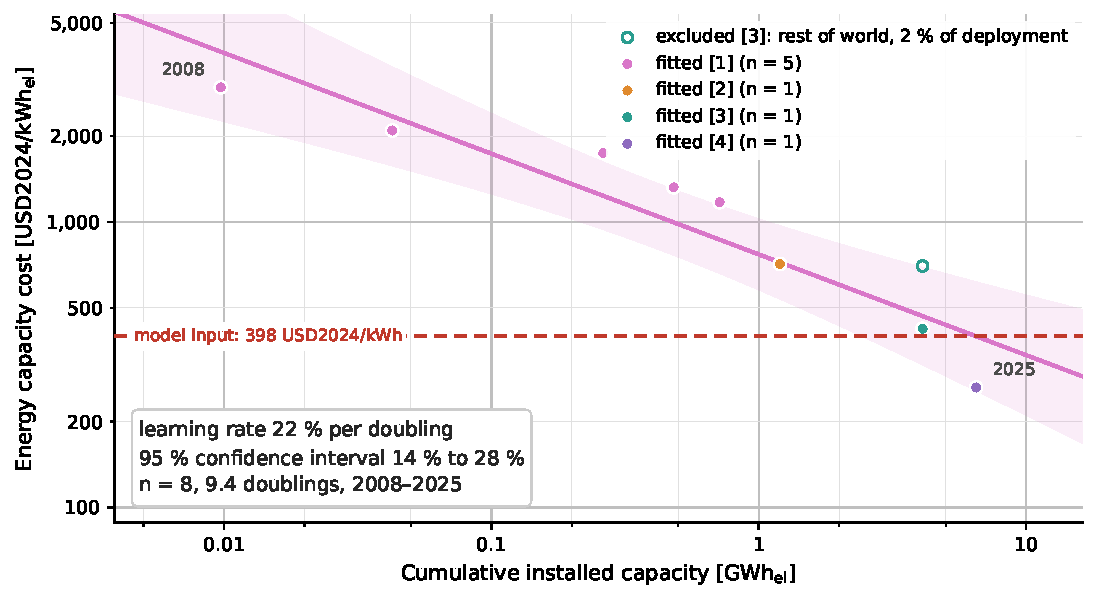
\includegraphics[width=\textwidth]{../../../misc-quarter1/technology-costs/figures/learning/vrfb.pdf}
\caption{Vanadium flow battery cost per kWh of storage against cumulative capacity.
Sources: [1] \citet{schmidt2018}; [2] Dalian Rongke, 100~MW / 400~MWh \citep{pvmag2022}; [3] installed system cost in China (filled) and in the rest of the world (hollow, 2\,\% of deployment, not fitted) from BNEF's 2024 survey \citep{esn2025}; [4] Rongke, 200~MW / 1~GWh in Xinjiang, supplier price \citep{projectblue2025}.
Cumulative capacity after 2017 counts Chinese additions only.
Dashed red line: the model input.}\label{fig:vrfb}
\end{figure}

The fixed O\&M of 4.7~\$/kW/yr plus 0.93~\$/kWh/yr over 8~hours and the 12-year lifetime come from technology-data \citep{technologydata}.
The table's efficiency of 0.806 is the value of technology-data \citep{technologydata} for one direction (charging or discharging); the round trip is 0.65.
Existing capacity is about 1~GW: roughly 4~GWh of flow batteries were installed by the end of 2024, mostly in China, at a typical duration of 4~hours (our compilation of \citet{schmidt2018} and recent project data).
The lead time is 1~year.
